%!TEX root = ../dissertation.tex


\chapter{\label{chap:halo}Neutrino Halo Problem}


One of the big questions about neutrino oscillations in supernovae is the so called halo problem. Cherry et al showed that neutrino flavor conversions are greatly affected by the back scattered neutrinos in supernovae~\cite{Cherry2012}. Neutrinos around supernovae are scattered and some of them are scattered to move almost backward. On the other hand, neutrino self-interactions is proportional to the inner product of momenta of neutrinos, which leads to the dependence on $1-\cos\theta$ where $\theta$ is the angles between momenta of two neutrinos. Most of the research has been concentrating on mostly forward scattering, with small values for $1-\cos\theta$. For back ward scattered neutrinos, the interaction potential can be much larger than the forward scattered neutrino contributions. Though the work by Sarikas et al showed that matter suppression is still significant within this region~\cite{Sarikas2012a}, it is not clear how exactly the neutrino halo alters neutrino oscillations. The halo problem itself is worth more calculations.


\section{\label{chap:halo-sec:line}Line Model}

We continue to use the simplified line model and build our intuitions out of it. The halo problem is simplified to have neutrinos emitted from a line $z=0$ homogeneously, which are reflected from a certain distance $z=L$. In principle, the reflection angles doesn’t have to be Snell’s law. The scattering can be in any angle with different amplitudes. Here I am using this very simple Snell’s law just to explore the effect of halo. It's crucial to keep an eye on the simplifications in this line model.
\begin{itemize}
    \item Neutrinos are emitted from a line, which is not the case in a real supernova.
    \item Neutrinos are emitted with translation symmetry on the line. Breaking the symmetry might bring in other qualitatively different results.
    \item Neutrinos are reflected from a certain surface $z=L$, which is different from reality where neutrinos are scattered everywhere.
    \item Neutrinos are reflected according to Snell's law.
    \item Neutrinos are homogeneously reflected at $z=L$.
\end{itemize}



\begin{figure}
    \centering
    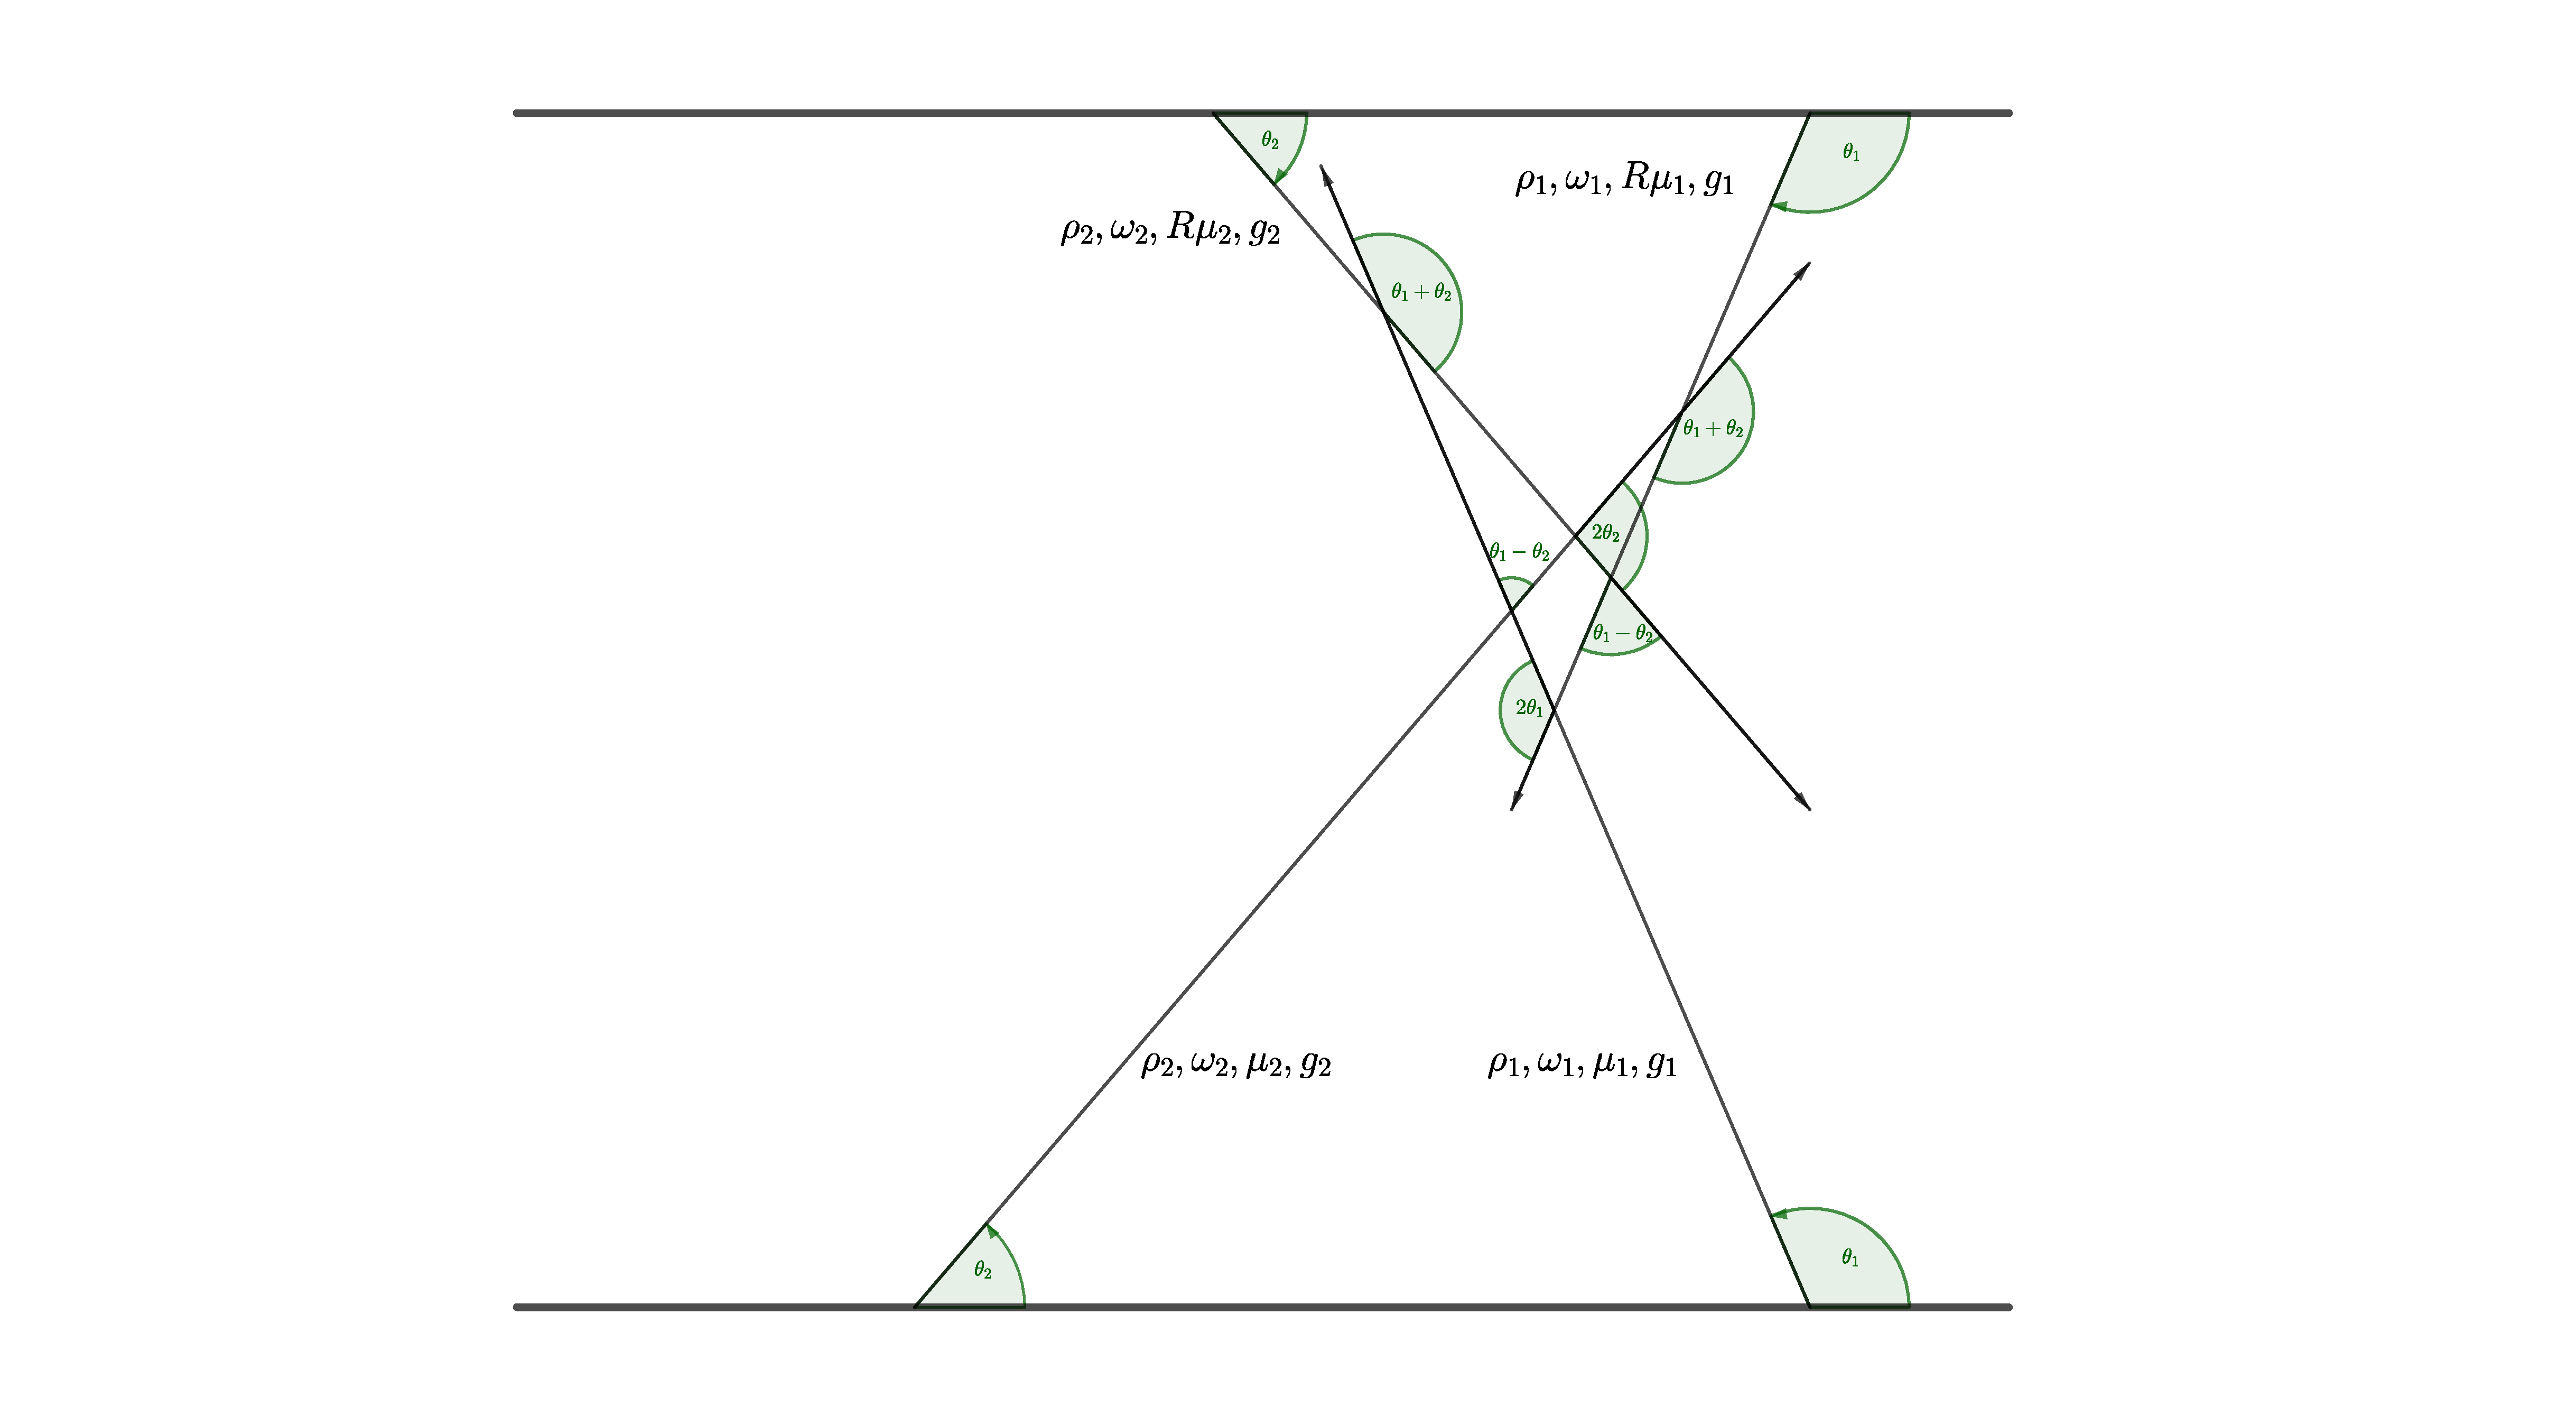
\includegraphics[width=\textwidth]{chapters/assets/halo/line-model.pdf}
    \caption{Line model used for halo problem. Neutrinos are emitted from the bottom line and reflected at the top line.}
    \label{chap:halo-sec:line-fig:line-model}
\end{figure}


The algorithm that I used is relaxation method. The algorithm is meant to find the equilibrium state of neutrino oscillations with the presence of halo.
\begin{enumerate}
\item Calculate forward beam using 0 backward beam;
\item Calculate backward beam using forward beam calculated in 1;
\item Calculate forward beam using backward beam calculated in 2;
\item Repeat until the beams reach equilibrium.
\end{enumerate}


\section{\label{chap:halo-sec:line-sym}Neutrino Beams Only}

As a first step, I calculated neutrino oscillations with only neutrino beams. Before we rush to the numerical results, I linearized the equation of motion and worked out the linear stability analysis.

In linear regime, we define the density matrices for forward and backward beams to be
\begin{align*}
   \rho_F &= \frac{1}{2} \begin{pmatrix}
   1 & \epsilon_F \\
   \epsilon_B^* & -1
   \end{pmatrix} \\
   \rho_B &= \frac{1}{2} \begin{pmatrix}
   1 & \epsilon_B \\
   \epsilon_B^* & -1
   \end{pmatrix}.
\end{align*}
The Hamiltonian for forward and back ward beams are
\begin{align*}
   H_F &= H_v + \mu \rho_F \\
   H_B &= H_v + R \mu \rho_B.
\end{align*}
We will investigate the instability for zero mixing angle for new instabilities. The linearized equation of motion can be simplified to
\begin{align*}
   i\partial_z \begin{pmatrix}
   \epsilon_F \\
   \epsilon_B
   \end{pmatrix} = \begin{pmatrix}
   -\omega_v + R \xi \mu & - R \xi \mu \\
   \xi \mu & \omega_v - \xi \mu
   \end{pmatrix} \begin{pmatrix}
   \epsilon_F \\
   \epsilon_B
   \end{pmatrix}.
\end{align*}
This equation can be easily solved. The eigenvalues are
\begin{align*}
   \Omega_+ &= \frac{1}{2} ( (R-1)\xi\mu + \sqrt{\Delta} ) \\
   \Omega_- &= \frac{1}{2} ( (R-1)\xi\mu - \sqrt{\Delta} ),
\end{align*}
where
\begin{equation}
   \Delta = (1-R)^2 \mu^2 \xi^2 - 4\mu\xi \omega_v (1+R) + 4\omega_v^2.
\end{equation}
The corresponding eigenvectors are
\begin{align*}
   V_+ &=\begin{pmatrix}
   \frac{ -2\omega_v + \xi \mu (1+R) + \sqrt{\Delta} }{2\xi\mu} \\
   1
   \end{pmatrix} \\
   V_- &=\begin{pmatrix}
   \frac{ -2\omega_v + \xi \mu (1+R) - \sqrt{\Delta} }{2\xi\mu} \\
   1
   \end{pmatrix}.
\end{align*}
The general solution to the equation is
\begin{equation*}
   \begin{pmatrix}
   \epsilon_F(z) \\
   \epsilon_B(z)
   \end{pmatrix} = C_+ V_+ e^{-i \Omega_+ z} +  C_- V_- e^{-i \Omega_- z}.
\end{equation*}

The special property about this reflection problem is that the density matrices for the forward and backward beams should be the same at the reflection point, say $z=L$. With such a simple relation, we can find the relations between $C_\pm$ by setting $\epsilon_F(L)=\epsilon_B(L)$,
\begin{equation}
   \frac{C_+}{C_-} = e^{-i(\Omega_- -\Omega_+)L} \frac{ \sqrt{\Delta} +  2\omega_v + \mu \xi (1-R) }{\sqrt{\Delta} -  2\omega_v - \mu \xi (1-R)}.
\end{equation}
The solution to be problem can be simplified,
\begin{equation}
   \begin{pmatrix}
   \epsilon_F(z) \\
   \epsilon_B(z)
   \end{pmatrix} = C_- e^{-i\Omega_- L} \left( \frac{ \sqrt{\Delta} +  2\omega_v + \mu \xi (1-R) }{\sqrt{\Delta} -  2\omega_v - \mu \xi (1-R)} V_+ e^{-i \Omega_+ (z-L)} +  V_- e^{-i \Omega_- (z-L)} \right).
\end{equation}

We are interested in the absolute values of each elements so that the overall factors can be neglected. The forward beam evolution is obtained by taking the absolute value of $\epsilon_F$,
\begin{align*}
   \left\vert \epsilon_F \right\vert \propto & \lvert (2\omega_v +\xi\mu(1-R) +i \delta ) ( -2\omega_v + \xi\mu(1+R) + i \delta ) e^{\delta(z-L)} \\ 
   &+ ( -2\omega_v - \xi\mu(1-R) +i \delta ) ( -2\omega_v + \xi\mu(1+R) - i \delta ) e^{-\delta(z-L)} \rvert,
\end{align*}
in which $\sqrt{\Delta}$ is replaced by $i \delta$. We collecting terms and verify that it has the form
\begin{equation}
   \left\vert \epsilon_F \right\vert \propto A + B \cosh( 2\delta(L-z) ),
\end{equation}
where $B\leq 0$.
The only $z$ dependent term is $\cosh( 2\delta(L-z) )$, which is decreasing within $[0,L]$ and is increasing in $[L,2L]$. The slope at $z=L$ is 0. An example is plotted in Fig.~\ref{chap:halo-sec:line-sym-fig:cosh}.


\begin{figure}
    \centering
    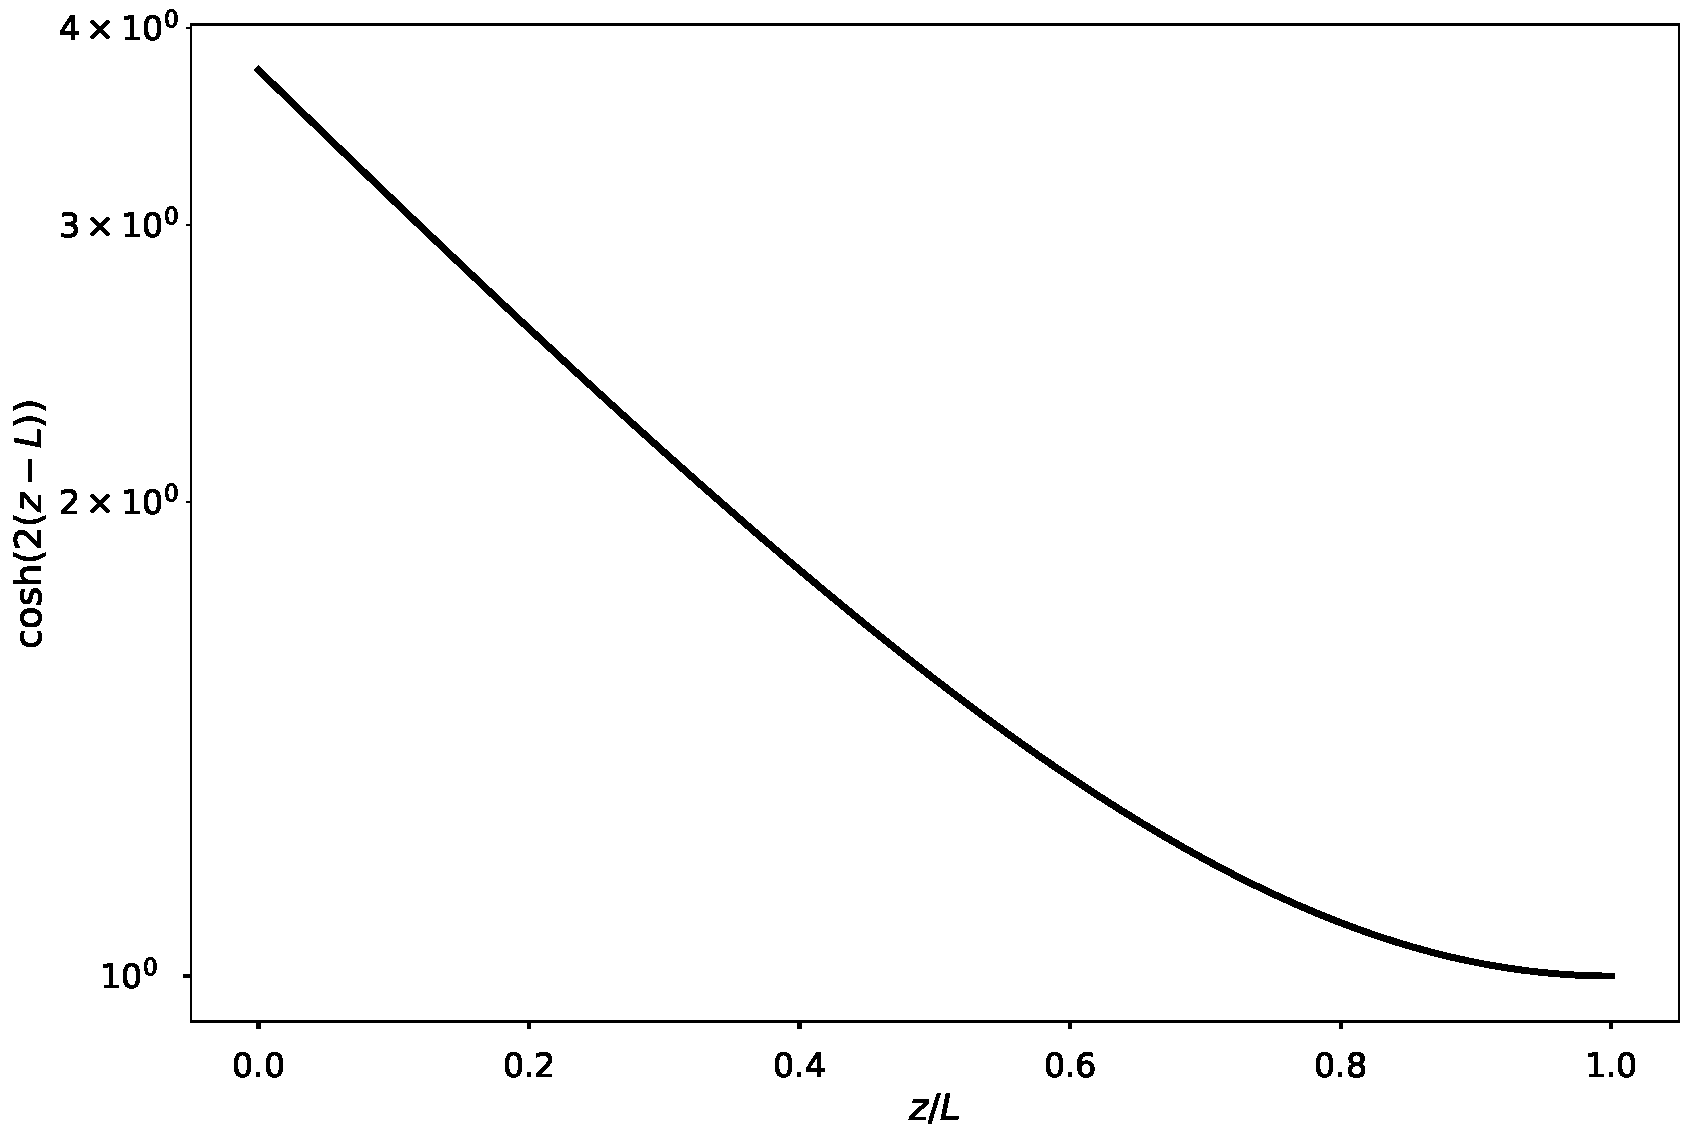
\includegraphics[width=\textwidth]{chapters/assets/halo/cosh.pdf}
    \caption{ An example of $\cosh(2\delta(z-L))$ with $\delta=1$, and $L=5$.}
    \label{chap:halo-sec:line-sym-fig:cosh}
\end{figure}


We expect the numerical calculations bare the same behavior that the instability leads to no growth but decrease in flavor conversion, assuming the neutrinos start from electron flavor. The result indeed confirms it, as shown in~Fig.~\ref{chap:halo-sec:line-sym-fig:mu-1.0-reflection-0.07}.

\begin{figure}
    \centering
    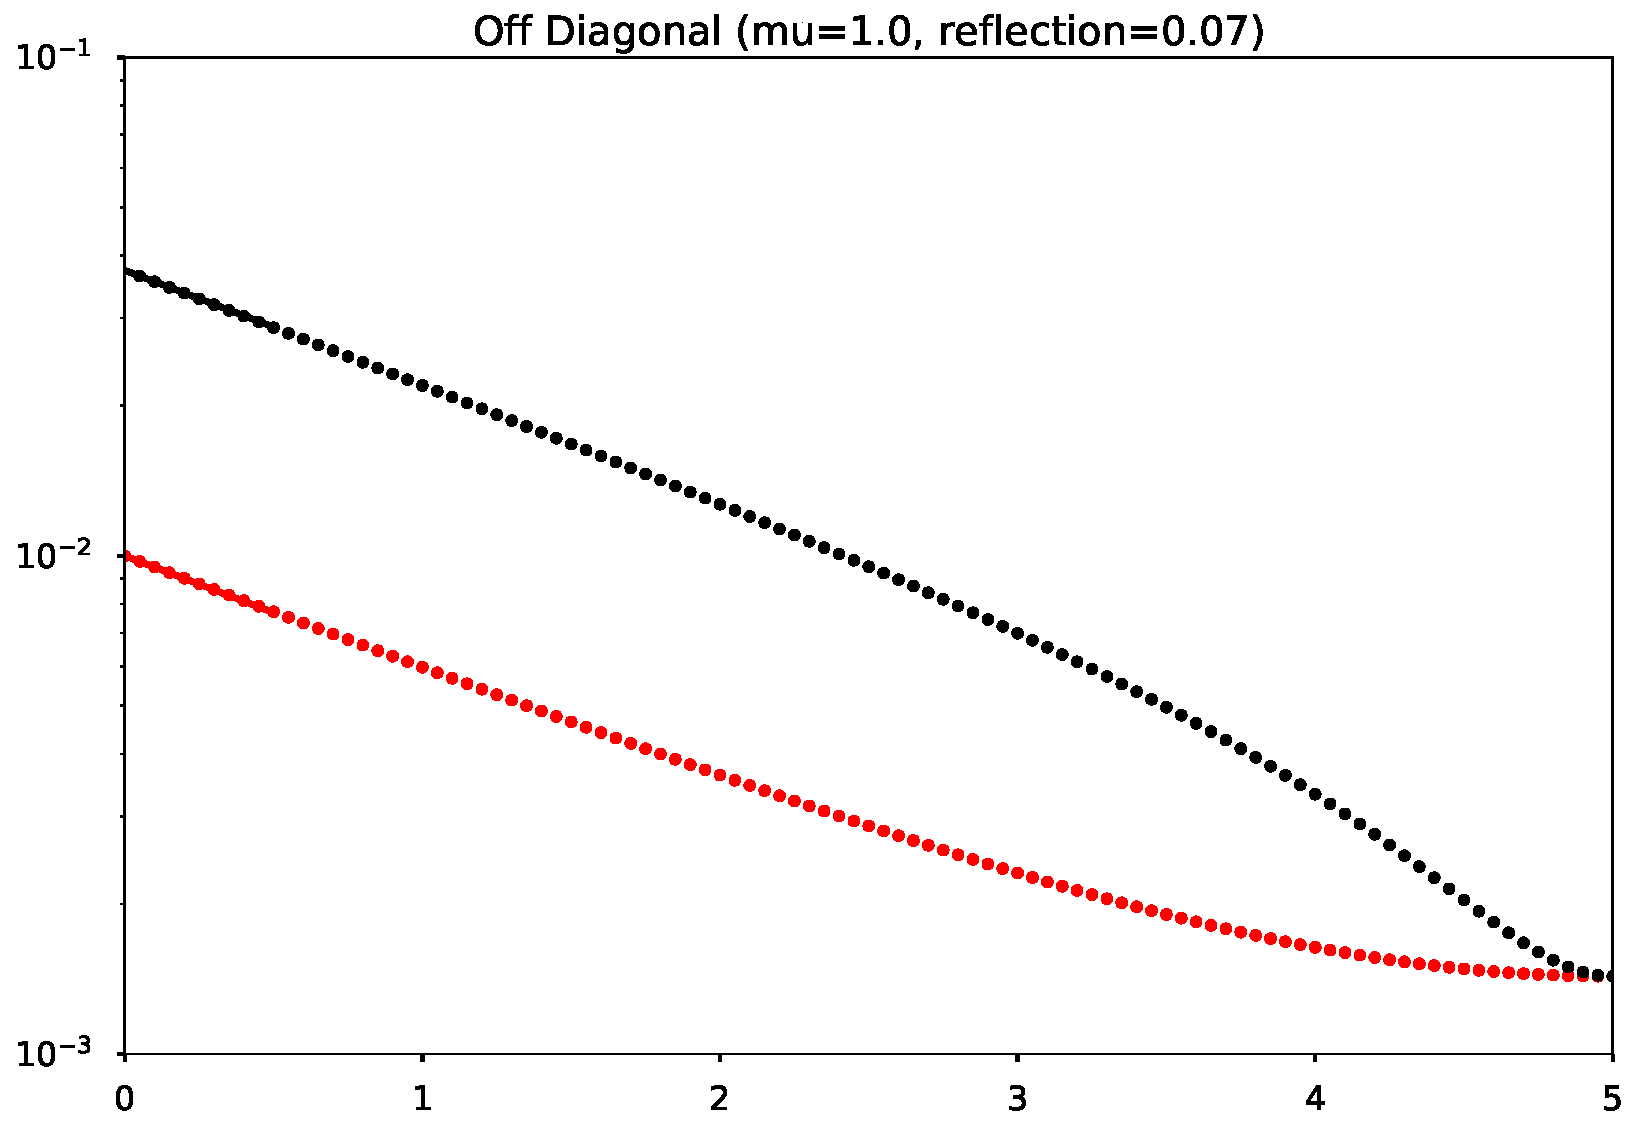
\includegraphics[width=\textwidth]{chapters/assets/halo/mu-1-reflection-0p07.pdf}
    \caption{Absolute value of off diagonal element for $\mu=1.0$, $R=0.07$, $L=5$. The red dots are for the forward beam and the black dots are for the backward beams. The lines are indicating the predictions of linear stability analysis.}
    \label{chap:halo-sec:line-sym-fig:mu-1.0-reflection-0.07}
\end{figure}

We compare this simplified halo problem with bipolar model.